\begin{exercise}
Betrachten Sie das System
\begin{align*}
  x^{\prime} &= y \\
  y^{\prime} &= x^2 + x.
\end{align*}
Zeigen Sie, dass $h(x,y) := y^2 - x^2 -\frac{2}{3}x^3$ eine Erhaltungsgröße ist.
Benutzen Sie diese Information, um das Phasenportrait zu skizzieren.
Was können Sie über die Stabilität der beiden Ruhelagen aussagen?
\end{exercise}
\begin{solution}
  Die Funktion $h$ ist eine Erhaltungsgröße, denn
  \begin{align*}
      \frac{\partial}{\partial t}h(x(t), y(t)) = 2y(t)y^\prime(t) - 2x(t)x^\prime(t)
       = 2y(t)(x^2(t) + x(t)) - 2x(t)y(t) -2x^2(t)y(t) = 0.
  \end{align*}
  Wir definieren die Funktion
  \begin{align*}
    f\left(\begin{pmatrix}
      x \\ y
    \end{pmatrix}\right) :=
    \begin{pmatrix}
      y \\ x^2 + x
    \end{pmatrix}
  \end{align*}
  und bestimmen die Ruhelagen
  \begin{align*}
    f\left(\begin{pmatrix}
      x \\ y
    \end{pmatrix}\right) =
    \begin{pmatrix}
      y \\ x^2 + x
    \end{pmatrix} \stackrel{!}{=}
    \begin{pmatrix}
      0 \\ 0
    \end{pmatrix}.
  \end{align*}
  Aus der ersten Gleichung erhalten wir $y = 0$
  und aus der zweiten
  \begin{align*}
    x^2 + x = (x + 1)x = 0 \iff x \in \{0,-1\}.
  \end{align*}
  Also haben wir zwei Ruhelagen
  \begin{align*}
    f \pbraces{
    \begin{pmatrix}
      x \\ y
    \end{pmatrix}}
    = 0 \Leftrightarrow
    \begin{pmatrix}
      x \\ y
    \end{pmatrix}
    =
    \begin{pmatrix}
      0 \\ 0
    \end{pmatrix}
    \lor
    \begin{pmatrix}
      x \\ y
    \end{pmatrix}
    =
    \begin{pmatrix}
      -1 \\ 0
    \end{pmatrix}.
  \end{align*}
  Damit können wir nun ein schönes Phasenportrait erstellen, indem wir im
  Hintergrund die Höhenlinien von $h$ plotten. Aufgrund der Erhaltungsgrößeneigenschaft
  von $h$ können Lösungen ihre jeweiligen Höhenlinien nie verlassen.
  \FloatBarrier
  \begin{figure}
      \centering
      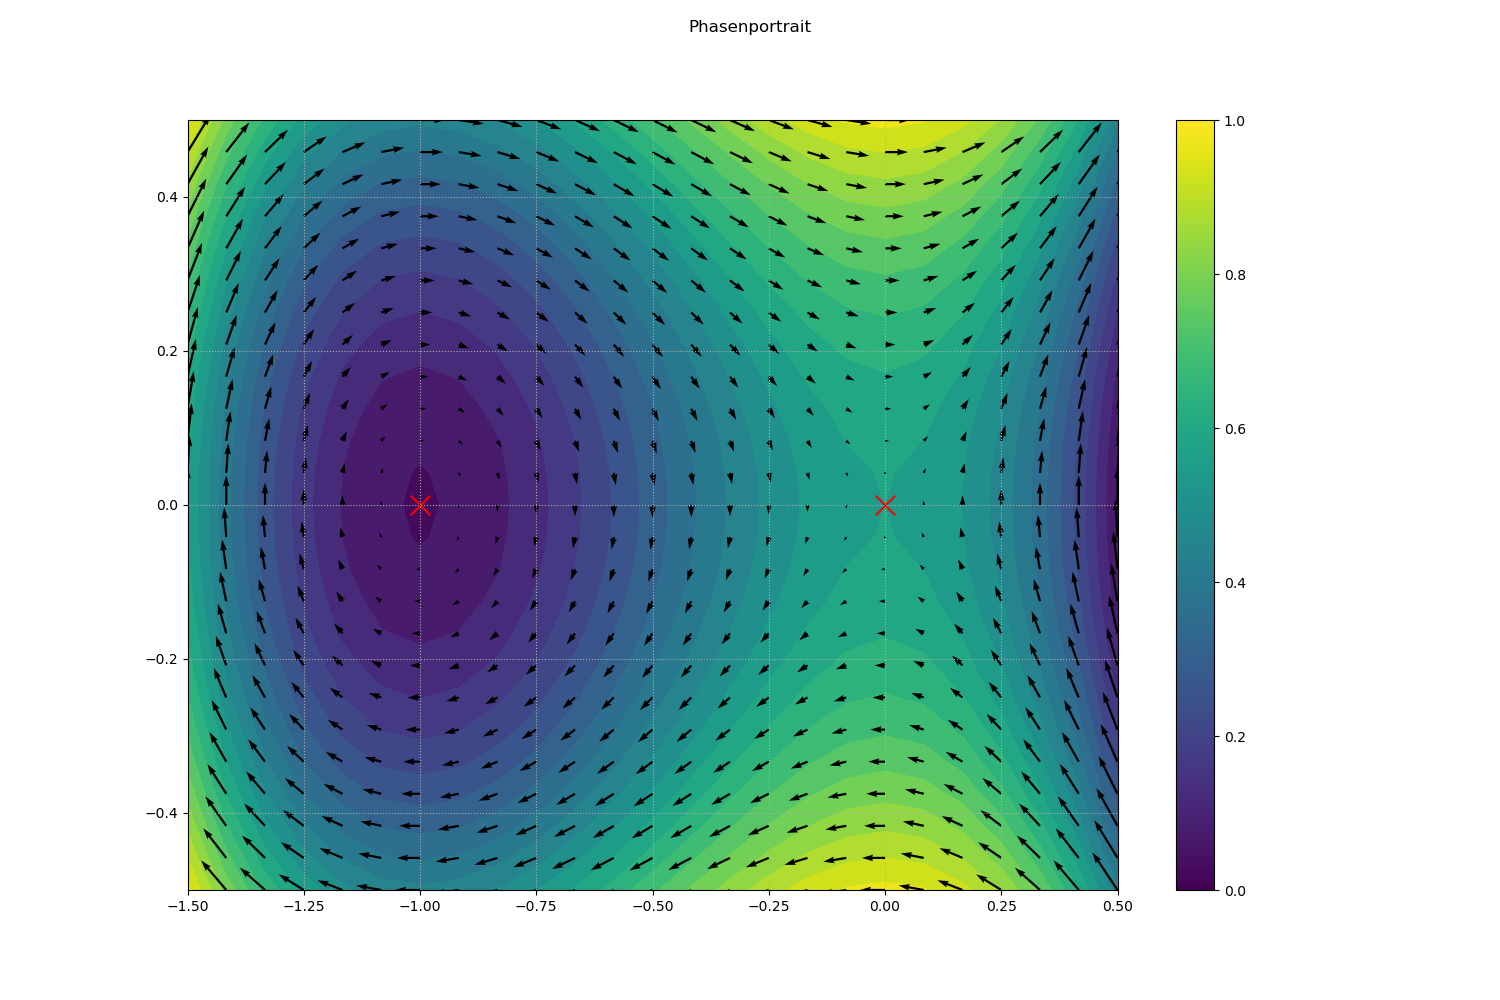
\includegraphics[width=\linewidth]{plot7.4.png}
  \end{figure}
  \FloatBarrier
  Das Phasenportrait lässt uns vermuten, dass $(-1,0)^{\top}$ eine asymptotisch stabile Ruhelage darstellt,
  während $(0,0)^{\top}$ instabil ist.
  Das gilt es nun formal zu überprüfen.
  \begin{itemize}
    \item $(0, 0)^T$: \\
    Wir berechnen die Ableitungsmatrix von $f$
    \begin{align*}
      Df\pbraces{\begin{pmatrix}
        x \\ y
      \end{pmatrix}}
      =
      \begin{pmatrix}
        0 & 1 \\
        2x+1 & 0
      \end{pmatrix},
      \quad \textrm{also} \quad
      Df\pbraces{\begin{pmatrix}
        0 \\ 0
      \end{pmatrix}}
      =
      \begin{pmatrix}
        0 & 1 \\
        1 & 0
      \end{pmatrix}
    \end{align*}
    Von dieser Matrix ist das charakteristische Polynom
    \begin{align*}
      \chi(\lambda) = \det \begin{pmatrix}
        -\lambda & 1 \\
        1 & -\lambda
      \end{pmatrix}
      = \lambda^2 - 1 \quad \textrm{und daher} \quad \chi(\lambda) = 0 \Leftrightarrow \lambda^2 - 1 = 0 \Leftrightarrow \lambda = \pm 1.
    \end{align*}
    Da ein Eigenwert positiv ist wissen wir nach Satz 5.8, dass es sich bei $(0, 0)^T$ um eine instabile Ruhelage handelt.
    \item $(-1, 0)^T$: \\
    Wir berechnen wieder die Ableitungsmatrix
    \begin{align*}
    Df\pbraces{\begin{pmatrix}
      -1 \\ 0
    \end{pmatrix}}
    =
    \begin{pmatrix}
      0 & 1 \\
      -1 & 0
    \end{pmatrix}
    \end{align*}
    mit dem charakteristischen Polynom
    \begin{align*}
      \chi(\lambda) = \lambda^2 + 1.
    \end{align*}
    Die Nullstellen davon lauten
    \begin{align*}
      \lambda_{1,2} = \pm i
    \end{align*}
    und diesmal liefert uns Satz 5.8. keine Aussage. \\
    Da wir allerdings wissen, dass Erhaltungsgrößen
    Ljapunovfunktionen sind, können wir noch mit der direkten Methode von Ljapunov
    überprüfen, ob mit $(-1,0)$
    ein striktes Minimum von $h$ vorliegt.
    \begin{align*}
      \frac{\partial}{\partial x}h(x,y) &= -2x - 2x^2 \\
       \frac{\partial}{\partial y}h(x,y) &= 2y
    \end{align*}
    Also erhalten wir in unserem Fall
    \begin{align*}
    \frac{\partial}{\partial x}h(-1,0) &= -2 + 2 = 0 \\
     \frac{\partial}{\partial y}h(-1,0) &= 0.
    \end{align*}
    Betrachten wir nun die zugehörige Hesse-Matrix
    \begin{align*}
      \begin{pmatrix}
        \frac{\partial^2 f }{\partial x^2} & \frac{\partial^2 f }{\partial x \partial y} \\
        \frac{\partial^2 f }{\partial y \partial x} & \frac{\partial^2 f }{\partial y^2}
      \end{pmatrix}
      =
      \begin{pmatrix}
        -2-4x & 0 \\
        0 & 2
      \end{pmatrix}.
    \end{align*}
    Setzen wir nun ein, erhalten wir mit
    \begin{align*}
    \begin{pmatrix}
      2 & 0 \\
      0 & 2
    \end{pmatrix}
    \end{align*}
    eine klarerweise positiv definite Matrix und somit ist $(-1,0)^{\top}$
    ein striktes Minimum der Ljapunovfunktion $h$ und somit stabil.
    $(-1,0)^{\top}$ ist zwar eine isolierte Ruhelage, aber da unsere
    Ljapunovfunktion entlang Lösungen konstant ist, kann sie nicht strikt
    sein und somit liefert uns Satz 5.19. keine Aussage darüber, ob die
    Ruhelage asymptotisch stabil ist oder nicht.
  \end{itemize}
\end{solution}
